% ==================================================================================================== PART II
\part{Kneser graphs: exact minrank and an agent that proves it}
\label{part:kneser}

% ---------------------------------------------------------------------------------------------------- 8
\section{Exact minrank of Kneser graphs}\label{sec:minrank}

\subsection{Index coding, minrank and Kneser graphs}
\textbf{Index coding~\cite{baryossef}.} A sender holds one message per receiver. Receiver $v$ wants its own message
and already knows the messages of its neighbours in a graph $G$. How few broadcasts suffice? For every field $F$,
\begin{equation}
  \underbrace{\alpha(G)}_{\text{lower bound}} \;\le\; \underbrace{\beta(G)}_{\text{optimum}} \;\le\;
  \underbrace{\operatorname{minrk}_F(G)}_{\text{best linear code}} \;\le\; \underbrace{\bar\chi(G)}_{\text{clique cover}}.
\end{equation}
Here $\alpha$ is the independence number (the most receivers with no side information about each other), $\beta$
the broadcast rate, $\operatorname{minrk}_F$ the minrank over $F$ (the least rank of a matrix that \emph{fits} $G$:
nonzero diagonal, zero on non-adjacent pairs), and $\bar\chi$ the clique cover number. The best scalar linear code
over $F$ has length $\operatorname{minrk}_F(G)$~\cite{baryossef}. Exact $\beta$ is known for very few graph families.

\begin{figure}[ht]
  \centering
  \begin{minipage}{0.36\textwidth}\centering
    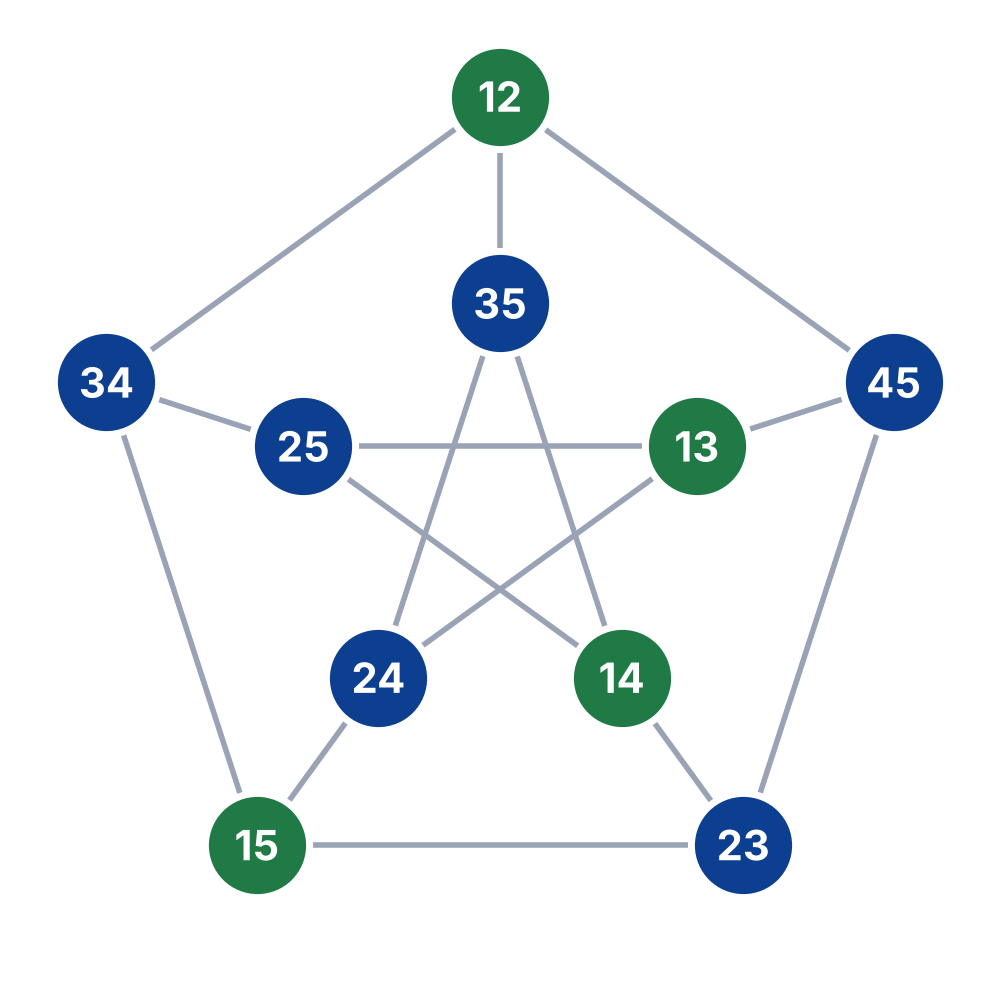
\includegraphics[width=\linewidth]{fig/k52.png}
  \end{minipage}\hfill
  \begin{minipage}{0.58\textwidth}
    \caption{The Kneser graph $K(5,2)$: 10 receivers (the pairs from $\{1,\dots,5\}$), two adjacent iff disjoint.
    Green: the 4 pairs containing 1. No two of them are adjacent, so $\alpha=4$: the Erd\H{o}s--Ko--Rado star.}
    \label{fig:k52}
  \end{minipage}
\end{figure}

\textbf{Kneser graph $K(n,k)$.} Receivers are all $k$-element subsets of $\{1,\dots,n\}$; two are adjacent iff
disjoint. By the Erd\H{o}s--Ko--Rado theorem~\cite{ekr}, $\alpha=\binom{n-1}{k-1}$, attained by the star $S=\{A: 1\in A\}$
(Figure~\ref{fig:k52}).

\subsection{The theorem}
Let $D$ be the disjointness (adjacency) matrix of $K(n,k)$, $\varepsilon=(-1)^{k-1}$ and $H=I+\varepsilon D$;
equivalently $H_{A,B}=\binom{|A\cap B|-1}{k-1}$. $H$ fits $K(n,k)$ over every field (it is the matrix of
Golovnev--Haviv~\cite{gh}, who bounded its rank by $\sum_{i<k}\binom{n}{i}$). For a prime $p$ let $q=q_p(k)$ be the
least power of $p$ with $q\ge k$.

\begin{theorem}\label{thm:rank}
For every prime $p$ and $n>2k\ge4$:
\[
  \operatorname{rank}_{\Fp}(I+\varepsilon D) = \binom{n-1}{k-1} \iff q_p(k) \mid n-2k .
\]
In particular, if $q\mid n-2k$ then $\operatorname{minrk}_{\Fp}(K(n,k))=\beta=\alpha$.
\end{theorem}

\begin{theorem}[explicit optimal index code]\label{thm:code}
If $q_p(k)\mid n-2k$, the following scalar linear code over $\Fp$ uses $\alpha=\binom{n-1}{k-1}$ transmissions,
optimal among all (also non-linear) index codes. For every $k$-set $A$ containing 1, broadcast
\[
  y_A = x_A + \varepsilon \sum_{B\cap A=\emptyset} x_B .
\]
A receiver $A\ni1$ decodes $x_A$ from $y_A$ (it knows every $x_B$ with $B$ disjoint from $A$). A receiver $A'\not\ni1$
computes $\varepsilon\sum_{A\ni1,\,A\cap A'=\emptyset} y_A = x_{A'}+\varepsilon\sum_{B\cap A'=\emptyset}x_B$ and
subtracts its side information.
\end{theorem}

\begin{corollary}[broadcast rate]
For every $k\ge2$ and all but finitely many $n$, $\beta(K(n,k))=\binom{n-1}{k-1}$, attained by a scalar linear code
over a suitable prime field. The field cannot be fixed in advance:
$\operatorname{minrk}_{\mathbb{F}_2}(K(7,2))=7>6=\operatorname{minrk}_{\mathbb{F}_3}(K(7,2))$.
\end{corollary}

\subsection{Proof}
Write $m=n-2k\ge1$.
\begin{enumerate}
  \item \textbf{Star rows are independent.} $H$ restricted to $S\times S$ is the identity (two members of $S$ share
  the element 1), so $\operatorname{rank}H\ge\alpha$ over every field.
  \item \textbf{Decoding identity.} For $A'\notin S$ and any $k$-set $B$, let
  $R(A',B)=\sum_{A\in S,\,A\cap A'=\emptyset}H_{A,B}$. If $1\in B$ then $\varepsilon R=H_{A',B}$. If $1\notin B$ then
  $\varepsilon R=\binom{m-1+t}{k-1}$ with $t=|A'\cap B|$, while $H_{A',B}=\binom{t-1}{k-1}$.
  \item \textbf{Rank $\alpha$ iff a congruence.} $\operatorname{rank}_p H=\alpha$ iff
  $\binom{m-1+t}{k-1}\equiv\binom{t-1}{k-1}\pmod p$ for $t=0,1,\dots,k$. ($\Leftarrow$: every row outside $S$ is
  $\varepsilon$ times the sum of the disjoint star rows. $\Rightarrow$: restricting to the star columns, where $H=I$,
  forces those coefficients, and every $t$ occurs.)
  \item \textbf{Lucas' theorem~\cite{lucas}.} With $g(x)=\binom{x+m}{k-1}-\binom{x}{k-1}=\sum_{i=1}^{k-1}\binom{m}{i}\binom{x}{k-1-i}$
  (Vandermonde), the congruences are equivalent to $\binom{m}{i}\equiv0\pmod p$ for $1\le i\le k-1$, which by Lucas'
  theorem holds iff $q_p(k)\mid m$.
\end{enumerate}
Since $H$ fits $K(n,k)$, $\operatorname{minrk}_{\Fp}\le\alpha$ in those cases; $\alpha$ is a lower bound for every
index code, so the linear code is optimal. \qed

A second, independent proof of the ``if'' direction via the integer diagonal forms of Ducey et al.~\cite{ducey},
and a third for $k=3$ via inclusion matrices, are in \file{proof.md} of the repository.

\subsection{Which cases are new}
Known before: for $k\mid n$, Baranyai's theorem~\cite{baranyai} partitions the $k$-sets into $\binom{n-1}{k-1}$ perfect matchings
(cliques), so $\operatorname{minrk}=\alpha$ over every field. \textbf{New:} the exact $p$-rank of $H$ with an
if-and-only-if condition, the explicit code and decoder, and infinitely many $n$ with $k\nmid n$ for every $k$, where
even the fractional clique cover exceeds $\alpha$. Construction: take a prime $p>k$ and $n=2k+pt$ with
$t\equiv1\pmod k$. \textbf{Not claimed:} anything about other fields, or $\operatorname{minrk}>\alpha$ when
$q\nmid n-2k$ (then this $H$ has rank above $\alpha$, nothing more). The theorem gives $\operatorname{minrk}=\alpha$ only in the
\emph{if} direction: when $q\nmid n-2k$, $\operatorname{minrk}$ can still equal $\alpha$ through another matrix. For
example $K(9,3)$ over $\mathbb{F}_2$: $q_2(3)=4$ does not divide $3$, yet $3\mid9$, so Baranyai's theorem gives
$\operatorname{minrk}_{\mathbb{F}_2}=\alpha$.

\textbf{Relation to Ducey et al.~\cite{ducey}.} Their integer diagonal forms of the subset-intersection matrices
$D-\lambda I$ (for $n\ge3k-1$) reduce $\operatorname{rank}_pH$ to a weighted sum of the ranks of $k+1$ small
integer matrices, and our second proof (\file{proof.md}, Appendix~A) starts from that reduction. Their paper does
not evaluate these ranks for $H$ or state when the sum equals $\alpha$. What is new here beyond it is: the closed
form, $\operatorname{rank}_pH=\alpha$ if and only if $q_p(k)\mid n-2k$, for every $n>2k$ (a proof from their forms gives only
the ``if'' direction); the elementary proof above, which does not use diagonal forms; and
the consequences for index coding, namely $\operatorname{minrk}=\beta=\alpha$, the explicit code and decoder, and the
cases with $k\nmid n$. Our search of the literature (\file{proof.md}, Remark~5.5) found no exact minrank or
broadcast-rate values for Kneser graphs beyond the $k\mid n$ case; it was a web search, not an exhaustive review.

\begin{table}[ht]
  \centering\small
  \begin{minipage}[t]{0.52\textwidth}\centering
    \begin{tabular}{@{}llrr@{}}
      \toprule
      Graph & Field & $\operatorname{minrk}=\alpha$ & Fractional cover \\
      \midrule
      $K(7,2)$  & $\mathbb{F}_3$ & 6   & 7 \\
      $K(10,3)$ & $\mathbb{F}_2$ & 36  & 40 \\
      $K(13,4)$ & $\mathbb{F}_5$ & 220 & 238.3 \\
      $K(15,4)$ & $\mathbb{F}_7$ & 364 & 455 \\
      \bottomrule
    \end{tabular}\par\smallskip
    (a) New cases with $k\nmid n$: no clique cover reaches $\alpha$.
  \end{minipage}\hfill
  \begin{minipage}[t]{0.44\textwidth}\centering
    \begin{tabular}{@{}cl@{}}
      \toprule
      $k$ & \makecell{$n$ with $k\nmid n$ covered\\by no prime} \\
      \midrule
      2 & 5 \\
      3 & 7, 8 \\
      4 & 9, 10, 11, 14 \\
      5 & 11, 12, 13, 14, 16, 22 \\
      6 & 13, 14, 15, 16, 17, 22, 27, 32 \\
      \bottomrule
    \end{tabular}\par\smallskip
    (b) The finitely many exceptions. Values with $k\mid n$\\ (e.g.\ 18, 24, 42, 72 for $k=6$) are left\\ out: Baranyai's theorem covers them.
  \end{minipage}
  \caption{Which cases the theorem settles.}
  \label{tab:newcases}
\end{table}

\subsection{Worked example: an optimal code for $K(7,2)$ over $\mathbb{F}_3$}
$K(7,2)$ has 21 receivers (pairs from $1..7$); $q_3(2)=3$ divides $7-4$, so Theorem~\ref{thm:rank} applies with
$\varepsilon=-1$. For each pair $A=\{1,j\}$ broadcast $y_A=x_A-\sum_{B\cap A=\emptyset}x_B\pmod3$: 6 broadcasts $=\alpha$,
against 7 for the clique-cover code and 7 for the best linear code over $\mathbb{F}_2$. Receiver $\{1,4\}$ knows every
$x_B$ with $B$ disjoint from it, so it reads $x_{14}$ from $y_{14}$. Receiver $\{2,3\}$ computes
$-(y_{14}+y_{15}+y_{16}+y_{17})=x_{23}-\sum_{B\cap\{2,3\}=\emptyset}x_B$ and removes the sum it knows. Checked
numerically on random messages. Over $\mathbb{F}_2$ no 6-broadcast linear code exists (SAT, DRAT-checked).

\subsection{Evidence and computer proofs}
\begin{itemize}
  \item 318 $(n,k,p)$ cases with $\binom nk\le2000$: the row identity $\iff\operatorname{rank}_pH=\alpha\iff q\mid
  n-2k$; the congruence of step 4 checked for $k\le12$, $p\le13$, $m=n-2k\le400$.
  \item 82 cases checked by two independent rank codes (FLINT and an own Gaussian elimination mod $p$),
  $\binom nk\le3500$, $k\le6$; 39 of them with $k\nmid n$.
  \item 6{,}666 cases of the second proof (integer diagonal forms) agree with Theorem~\ref{thm:rank} ($k\le12$,
  $n\le120$, $p\le13$).
  \item $K(7,2)$ over $\mathbb{F}_2$: rank $\le6$ refuted by SAT; the UNSAT proof checked by drat-trim (0.39\,s).
  \item $\operatorname{minrk}_{\mathbb{F}_2}(K(7,3))=18$ and $\operatorname{minrk}_{\mathbb{F}_2}(K(8,3))=22$, above
  $\alpha=15$ and 21 (DRAT-checked; $K(8,3)$ at rank 21: solve 950\,s, check 1{,}663\,s).
  \item Open: $K(9,2)$ and $K(11,2)$ over $\mathbb{F}_2$; a star-basis SAT reduction (0.3\,s on $K(7,2)$, over 1\,h
  before) did not finish in 2\,h.
\end{itemize}

% ---------------------------------------------------------------------------------------------------- 9
\section{The Kneser agent: an LLM agent that proves the broadcast rate}\label{sec:agent}

\subsection{Why an agent?}
\begin{itemize}
  \item \textbf{Proving $\beta$ gets slow.} Standard methods (the CP-SAT constraint solver~\cite{cpsat} for $\alpha$ and
  the clique cover, the fractional cover, and $\mathbb{F}_2$ minrank by SAT) prove 2 of 25 benchmark graphs in 60\,s each. One
  certified rank check costs about $N^2r$: on $N=14{,}950$ receivers, 54\,s.
  \item \textbf{Real inputs arrive unlabelled:} vertices shuffled, no family name. The theorem helps only if someone
  recognises the structure and picks the right field and constant.
  \item \textbf{Idea.} An LLM reads a numeric summary of the graph, guesses its structure and plans which certified
  checks to run. A pool of worker processes runs the checks; the run stops the moment lower bound $=$ upper bound.
  Only certified results count, and an independent verifier re-checks the final code. The LLM never writes a bound.
\end{itemize}

\textbf{Baseline: the Kneser agent without an LLM} (Kushagra's script, Figure~\ref{fig:baseline}). A fixed sequence:
recognise $(n,k)$ from the vertex count and degree; the theorem names the prime; one exact rank (FLINT~\cite{flint})
gives the code length; a greedy independent set gives the lower bound; anything that does not certify goes to a
general minrank solver, so a wrong guess can never produce a wrong answer. The greedy step runs only on a recognised
Kneser graph: on any other graph the script goes straight to the general solver and reports that solver's bounds.

\begin{figure}[ht]
  \centering
  \begin{tikzpicture}[font=\footnotesize, >={Stealth[length=2mm]}, node distance=5mm,
      s/.style={rectangle, rounded corners=2pt, draw=black!60, fill=black!3, align=center, text width=2.45cm,
                minimum height=1.25cm, inner sep=2pt}]
    \node[s] (a) {\textbf{1. Recognise}\\$N=\binom nk$ and every degree $=\binom{n-k}{k}$};
    \node[s, right=of a] (b) {\textbf{2. Choose field}\\theorem names $p$; none $\to$ step 5};
    \node[s, right=of b] (c) {\textbf{3. Upper bound}\\$\operatorname{rank}_p(I+\varepsilon A)$, one FLINT rank};
    \node[s, right=of c] (d) {\textbf{4. Lower bound}\\greedy independent set (recognised graphs); equal $\Rightarrow$ proven};
    \node[s, right=of d] (e) {\textbf{5. Fallback}\\general minrank solver};
    \draw[->] (a) -- (b); \draw[->] (b) -- (c); \draw[->] (c) -- (d); \draw[->] (d) -- (e);
  \end{tikzpicture}
  \caption{The baseline Kneser agent (no LLM): five fixed steps, full exact rank ($O(N^3)$).}
  \label{fig:baseline}
\end{figure}

\subsection{Architecture of our agent}\label{sec:arch}

Figure~\ref{fig:arch} shows the architecture. Two kinds of component alternate: LLM roles (dark) that only decide
\emph{what to check}, and code (light) that computes and certifies every number. The verdict comes from the checks,
not from an LLM.

\begin{figure}[p]
  \centering
  \begin{tikzpicture}[
      font=\small, >={Stealth[length=2.4mm]},
      box/.style={rectangle, rounded corners=3pt, align=center, text width=4.0cm, minimum height=1.75cm, inner sep=4pt},
      llmb/.style={box, fill=llm, text=white},
      code/.style={box, draw=iitb!70, fill=codebox},
      resbox/.style={box, fill=okgreen, text=white},
      d/.style={font=\footnotesize},
      lab/.style={font=\footnotesize, align=center, text=black!80, inner sep=1.5pt}]
    % row A
    \node[code] (g) at (0,0) {\textbf{Input graph}\\[1pt]{\footnotesize adjacency matrix only;\\vertices shuffled, no name}};
    \node[code] (s) at (5.2,0) {\textbf{Summary + greedy bounds}\\[1pt]{\footnotesize $N$, degrees, regularity,
      common neighbours, triangles, integer spectrum; first $L$ and $U$}};
    % row B
    \node[llmb] (so) at (5.2,-3.4) {\textbf{Solver (LLM)}\\[1pt]{\footnotesize family hypothesis with evidence,
      plan of tool calls}};
    \node[llmb] (cr) at (10.4,-3.4) {\textbf{Critic (LLM)}\\[1pt]{\footnotesize accepts the plan or objects\\(up to 3 rounds)}};
    % row C
    \node[code, text width=9.2cm, minimum height=1.5cm] (val) at (7.8,-6.1) {\textbf{Reply validation (code)}\\[1pt]
      {\footnotesize JSON schema, known tool names, integer arguments, $p$ prime; every evidence number must be one the
      agent was given; every ``$C(a,b)=X$'' recomputed. Invalid: returned once with the error; second failure:
      deterministic default plan.}};
    % row D
    \node[code, minimum height=3.4cm] (rk) at (0,-9.7) {\textbf{Rank engine (code)}\\[1pt]{\footnotesize exact
      $\operatorname{rank}_p$ by rank factorisation $M=C\,M[S,:]$, early stop at $U-1$; $O(N^2r)$ with numba, FLINT and
      BLAS}};
    \node[code, minimum height=3.4cm] (tl) at (5.2,-9.7) {};
    \node[anchor=north, text width=3.9cm, align=left, font=\footnotesize] at ([yshift=-3pt]tl.north)
      {\centering\textbf{\small Tool library (code)}\par\smallskip
       \texttt{spectral}: $I+cA$ over $\Fp$,\\ \quad$(p,c)$ from the spectrum\\
       \texttt{try\_code}: any $(p,c)$\\
       \texttt{family\_rule}: the theorem\\
       \texttt{independent\_set}\\
       \texttt{binomial\_match}\\
       \texttt{hoffman}: information only};
    \node[code, minimum height=3.4cm] (sch) at (10.4,-9.7) {};
    \node[anchor=north, text width=3.9cm, align=center] at ([yshift=-3pt]sch.north)
      {\textbf{Scheduler (code)}\\[1pt]{\footnotesize runs the accepted plan on a pool of 3 worker processes}};
    \foreach \i/\xx in {1/9.05, 2/10.4, 3/11.75}
      \node[rectangle, draw=iitb!60, fill=white, minimum width=1.15cm, minimum height=0.55cm, font=\scriptsize]
        at (\xx,-10.9) {worker};
    % row E
    \node[llmb] (vl) at (0,-14.0) {\textbf{Verifier (LLM)}\\[1pt]{\footnotesize writes the analysis; may request
      extra checks}};
    \node[code] (ve) at (5.2,-14.0) {\textbf{Verifier (independent code)}\\[1pt]{\footnotesize checks the fit and the exact factorisation, runs its own elimination, decodes every receiver}};
    \node[code] (bd) at (10.4,-14.0) {\textbf{Bound board (code)}\\[1pt]{\footnotesize only certified results:
      $L\le\beta\le U$ (independent set re-checked; length = exact rank)}};
    % row F
    \node[resbox] (o) at (5.2,-16.8) {\textbf{Output}\\[1pt]{\footnotesize $\beta$, an optimal code and the full trace}};
    % arrows
    \draw[->] (g) -- (s);
    \draw[->] (s) -- (so);
    \draw[->] ([yshift=3mm]so.east) -- ([yshift=3mm]cr.west);
    \draw[->] ([yshift=-3mm]cr.west) -- ([yshift=-3mm]so.east);
    \draw[->] (so.south) -- (so.south |- val.north);
    \draw[->] (cr.south) -- (cr.south |- val.north);
    \draw[->] (val.south -| sch.north) -- node[lab, right] {accepted plan} (sch.north);
    \draw[<->] (tl.east) -- node[lab, above] {calls} (sch.west);
    \draw[->] (tl.west) -- node[lab, above] {ranks} (rk.east);
    \draw[->] ([xshift=-8mm]sch.south) -- node[lab, left, text width=1.7cm, align=right] {certified results}
      ([xshift=-8mm]bd.north);
    \draw[->, densely dotted, thick] ([xshift=8mm]bd.north) -- node[lab, right] {events} ([xshift=8mm]sch.south);
    \draw[->] (bd.west) -- node[lab, above] {$L=U$} (ve.east);
    \draw[<->] (ve.west) -- (vl.east);
    \draw[->] (ve.south) -- (o.north);
    \draw[->, dashed, thick, black!70] (bd.east) -- (13.5,-14.0) -- node[lab, rotate=90, below, pos=0.5]
      {checkpoint (once): plan exhausted and bounds still apart $\to$ the Solver revises the plan}
      (13.5,-1.75) -- (5.2,-1.75) -- (so.north);
  \end{tikzpicture}
  \par\medskip
  {\footnotesize
   \tikz\fill[llm] (0,0) rectangle (0.35,0.22);~LLM role \qquad
   \tikz{\fill[codebox] (0,0) rectangle (0.35,0.22); \draw[iitb!70] (0,0) rectangle (0.35,0.22);}~code \qquad
   \tikz\fill[okgreen] (0,0) rectangle (0.35,0.22);~result \qquad
   dashed: checkpoint loop\\[2pt] dotted: scheduler events (new bound $\to$ retarget; near miss $\to$ more constants for that field; $L=U$ $\to$ stop)}
  \caption{Architecture of the Kneser agent. The LLMs (Solver, Critic, Verifier) only decide what to check and explain
  the result; every number on the bound board is a certificate computed by code, and the final verdict comes from
  independent checking code that shares nothing with the tools. If the LLM's plans leave the bracket open after the
  checkpoint, a deterministic generic search still runs (safety net). The LLM is called only at the start, at the
  checkpoint and at the end.}
  \label{fig:arch}
\end{figure}

\textbf{Components.}
\begin{enumerate}
  \item \textbf{Input.} Only the adjacency matrix; the benchmark relabels the vertices with a random permutation
  (\texttt{--seed}) and never passes the graph's name.
  \item \textbf{Summary and greedy bounds (code).} Number of receivers, degree sequence, regularity, sampled
  common-neighbour counts, triangle count, and the integer spectrum with multiplicities. A greedy independent set and
  a greedy cover give the first bracket $[L,U]$ before any LLM call.
  \item \textbf{Solver and Critic (LLMs).} The Solver reads the summary and writes a family hypothesis with evidence
  (numbers from the summary) and a plan of tool calls; the Critic accepts it or objects, for up to 3 rounds. The
  system prompts are in Appendix~\ref{app:prompts}.
  \item \textbf{Reply validation (code).} Every LLM reply is checked: JSON schema, known tool names, integer
  arguments, $p$ prime; every evidence item must quote a number the agent was given, and every ``$C(a,b)=X$'' is
  recomputed. An invalid reply is returned once with the error; a second failure falls back to a deterministic default
  plan.
  \item \textbf{Scheduler and worker pool (code).} Runs the accepted plan on 3 worker processes and reacts to
  events: a new bound retargets the remaining checks; a near miss (rank just above $L$) tries more constants for the
  same field; $L=U$ stops everything at once; an exhausted plan triggers one checkpoint back to the Solver, which sees
  the results and revises the plan.
  \item \textbf{Tool library (code).} \texttt{spectral} (the generic rule: codes $M=I+cA$ over $\Fp$ with $(p,c)$
  ranked from the integer spectrum, $c=-1/\theta \bmod p$, predicted rank $N$ minus the multiplicity of eigenvalues
  $\equiv\theta$), \texttt{try\_code} (any $(p,c)$), \texttt{family\_rule} (Theorem~\ref{thm:rank}, one $(p,c)$ for
  $K(n,k)$; can be disabled), \texttt{independent\_set} (more greedy restarts), \texttt{binomial\_match} (find
  $(n,k)$ with $N=\binom nk$ and degree $\binom{n-k}{k}$), \texttt{hoffman} (Hoffman bound, information only).
  \item \textbf{Rank engine (code).} Exact $\operatorname{rank}_p(M)$ by rank factorisation with early stop:
  (i) eliminate a sample block $M[S_0,J]$ in numba to get rows $S$ and columns $Q$ with $M[S,Q]$ invertible, stopping
  once more than \texttt{cap} independent rows are found; (ii) invert $M[S,Q]$ with FLINT and set
  $C=M[:,Q]\,M[S,Q]^{-1}$; (iii) compute the residual $M-C\,M[S,:]$ in float64 BLAS blocks (exact, since every entry
  is $<p$ and $r(p-1)^2<2^{53}$); add any row with a nonzero residual and repeat. When every residual is zero,
  $\operatorname{rank}_p(M)=|S|$ exactly. With $\texttt{cap}=U-1$ a code that cannot improve the upper bound is
  abandoned early. Cost $O(N^2r)$ instead of FLINT's $O(N^3)$.
  \item \textbf{Bound board (code).} Only certified results can enter: \texttt{offer\_lower} re-checks the
  independent set; code lengths come from exact ranks.
  \item \textbf{Verifier.} Independent code (it imports nothing from the tools or the rank engine, which a test
  asserts) checks that the code fits the graph, the exact factorisation $M=M[:,S]\,M[S,:]$, its own elimination, and
  simulates decoding for every receiver. The Verifier LLM writes the analysis and may request extra checks.
  \item \textbf{Trace.} Every event, LLM message and board change is logged with a timestamp; proven codes are saved.
\end{enumerate}

\begin{table}[ht]
  \centering\small
  \begin{tabularx}{\textwidth}{@{}>{\raggedright\arraybackslash}p{2.3cm}>{\raggedright\arraybackslash}p{5.0cm}X@{}}
    \toprule
    & Kneser agent (no LLM) & Our LLM agent \\
    \midrule
    Input & adjacency matrix & same matrix, vertices shuffled; the LLM sees only a numeric summary \\
    Decision & 5 fixed steps & Solver LLM: hypothesis + plan; Critic LLM challenges it (up to 3 rounds) \\
    Field choice & from the theorem only & theorem as one tool, plus a generic rule from the eigenvalues and any $(p,c)$ \\
    Execution & one step after another & worker pool (3 processes); stops as soon as the bounds meet \\
    Wrong guess & fall back to the general solver & checkpoint: the Solver sees the results and revises the plan \\
    Rank check & full exact rank, $O(N^3)$ & rank factorisation with early stop, $O(N^2r)$ \\
    Checking & certificates re-checked in the same code & independent verifier code (shares nothing with the tools) \\
    Fixed cost & none (0.02\,s on small graphs) & LLM thinking, median 30\,s per graph (12--50\,s) \\
    \bottomrule
  \end{tabularx}
  \caption{The two agents compared.}
  \label{tab:agents}
\end{table}

\subsection{Results: time to prove $\beta$}\label{sec:agentres}
\textbf{Benchmark.} 25 graphs: 20 benchmark graphs, namely 14 regular Kneser graphs ($K(21,2)$, $K(29,2)$, $K(40,2)$, $K(53,2)$, $K(12,3)$,
$K(13,3)$, $K(16,3)$, $K(18,3)$, $K(21,3)$, $K(13,4)$, $K(15,4)$, $K(16,4)$, $K(17,4)$, $K(15,5)$), 3 exceptions of
the theorem ($K(10,4)$, $K(14,4)$, $K(13,5)$) and 3 controls ($K(16,4)$ and $K(18,3)$ each minus 1\% of their edges,
and a random 6-regular graph on 1{,}000 vertices); plus 5 large Kneser graphs $K(20,4)$ (4{,}845 receivers), $K(17,5)$
(6{,}188), $K(23,4)$ (8{,}855), $K(24,4)$ (10{,}626) and $K(26,4)$ (14{,}950). Seed 0, vertices shuffled. Time is the
wall time until the certified bounds first meet, LLM time included. Each run is pinned to one CPU core of a 4-core
container: the gain comes from the right code and a cheaper rank check, not from parallelism. Claude LLM time is the
wall time of a Claude Code agent answering request files (tool calls included), so it overstates pure model time.

\begin{figure}[ht]
  \centering
  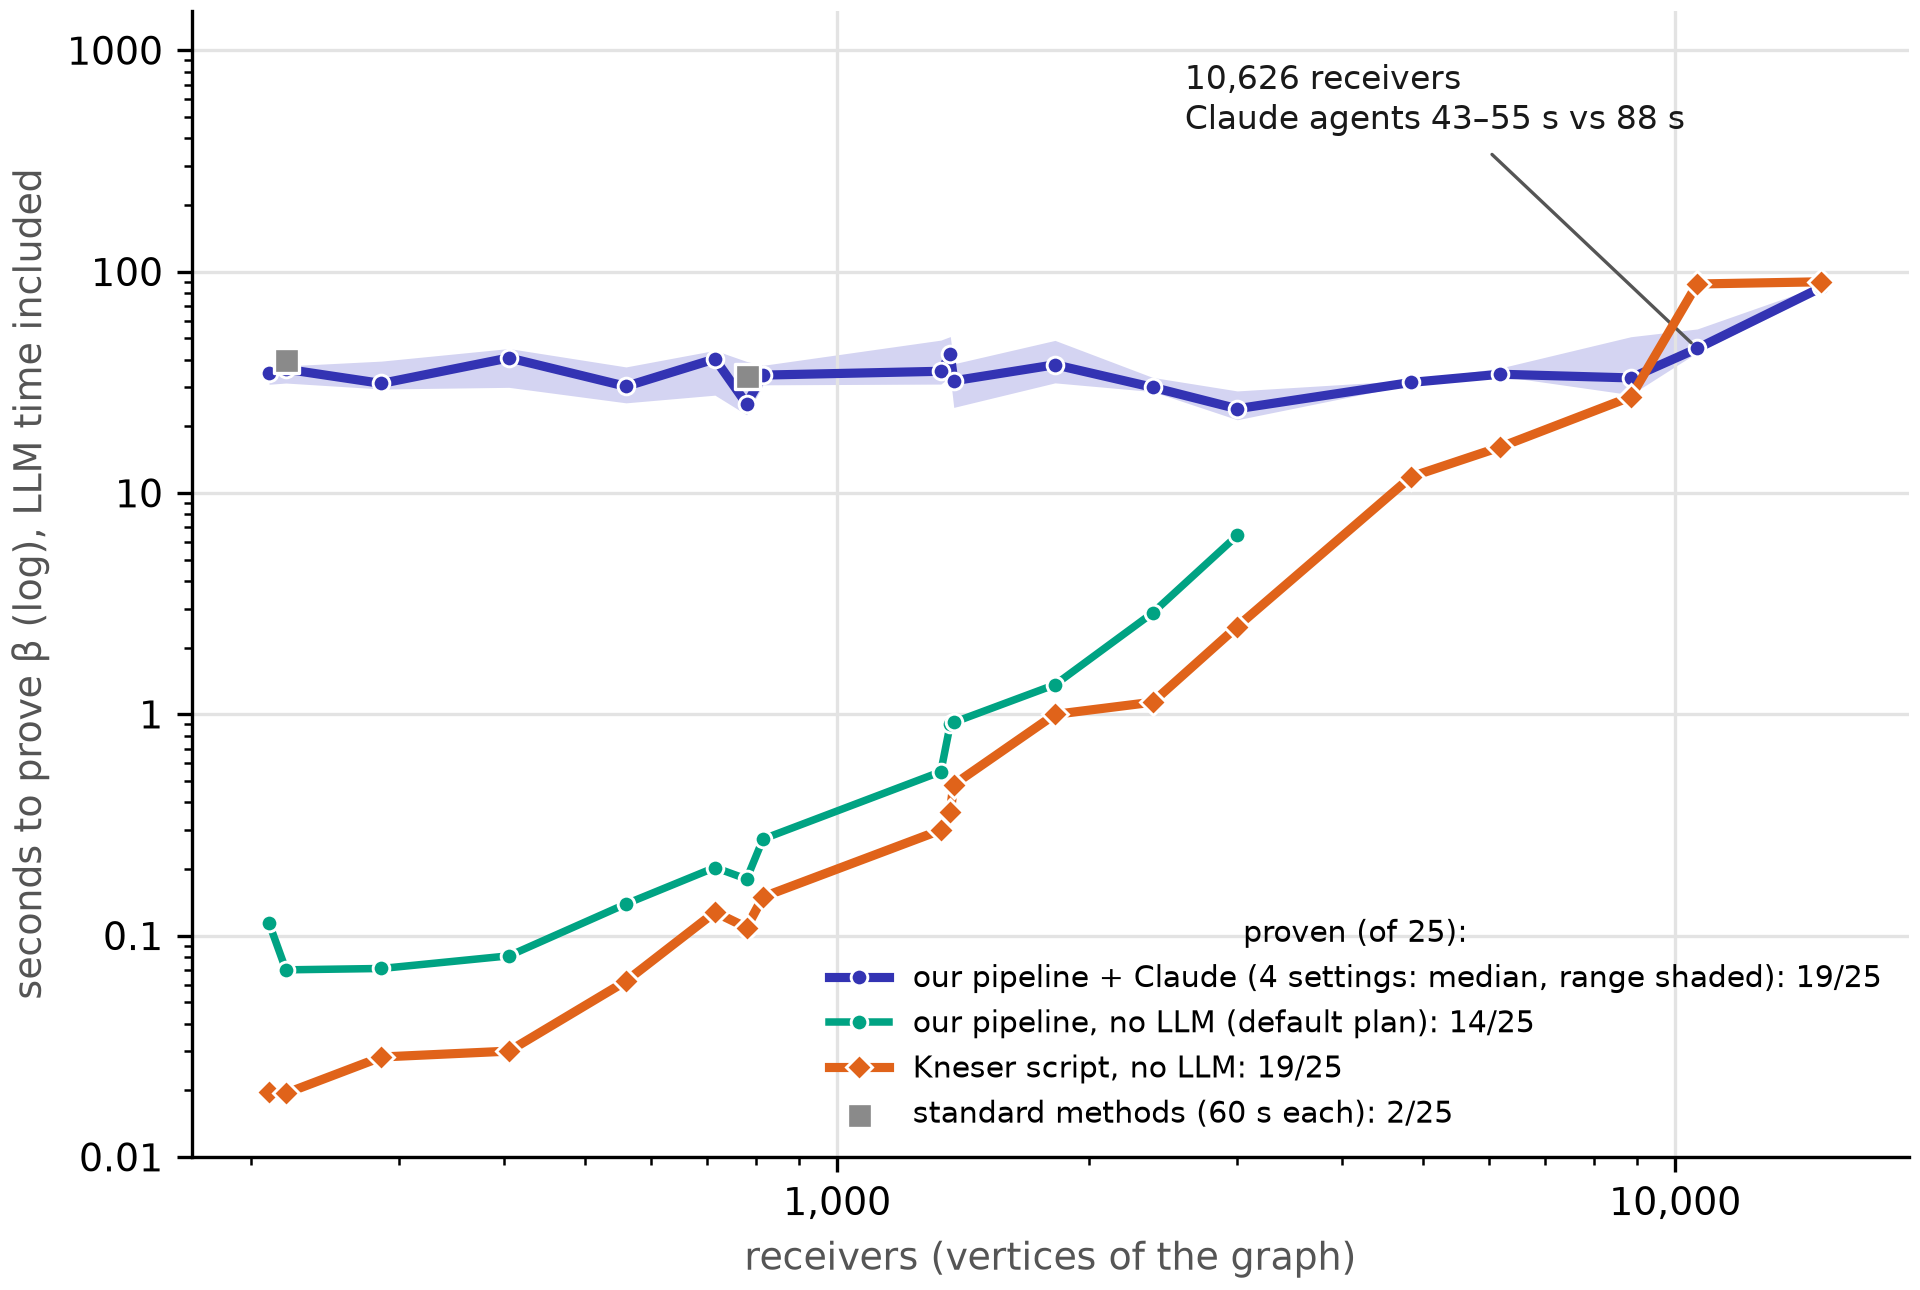
\includegraphics[width=0.82\textwidth]{fig/time_to_prove_beamer.png}
  \caption{Time to prove $\beta$ against the number of receivers (container, one CPU core per run, only proven graphs
  drawn): our pipeline with Claude (four settings), the same pipeline without an LLM (default plan), the no-LLM
  Kneser script, and the standard methods. Below about 9{,}000 receivers the script is faster; at 10{,}626 receivers
  the Claude agents need 43--55\,s against 88\,s, at 14{,}950 they need 81--87\,s against 90\,s. Without an LLM the
  default plan proves none of the five large graphs.}
  \label{fig:ttp}
\end{figure}

\begin{table}[ht]
  \centering\small
  \resizebox{\textwidth}{!}{\begin{tabular}{@{}lcccc@{}}
    \toprule
    & & & \multicolumn{2}{c}{Time at $N$ receivers} \\ \cmidrule(l){4-5}
    Method & Proven & Median time & 10{,}626 & 14{,}950 \\
    \midrule
    Standard methods (CP-SAT, covers, $\mathbb{F}_2$ SAT) & 2/25 & 40\,s & -- & -- \\
    Kneser script, no LLM & 19/25 & 0.36\,s & 87.9\,s & 89.9\,s \\
    \midrule
    Our pipeline, no LLM (default plan) & 14/25 & 0.24\,s & \makecell{open, $[1771,1948]$\\after 21.5\,s} & \makecell{open, $[2300,2529]$\\after 79.6\,s} \\
    \makecell[l]{Our pipeline, no LLM, fast path\\(GPU server; 23 graphs)} & 17/23 & 0.35\,s & not run & not run \\
    \midrule
    Our pipeline + Claude Sonnet 5.5 (medium) & 19/25 & 31.5\,s & 45.5\,s & 83.5\,s \\
    Our pipeline + Claude Opus 5.5 (low)      & 19/25 & 31.0\,s & 44.4\,s & 86.7\,s \\
    Our pipeline + Claude Opus 5.5 (medium)   & 19/25 & 35.9\,s & \textbf{43.1\,s} & \textbf{81.1\,s} \\
    Our pipeline + Claude Opus 5.5 (high)     & 19/25 & 38.3\,s & 55.0\,s & 86.2\,s \\
    \makecell[l]{Our pipeline + Qwen2.5-Coder-32B-AWQ\\(GPU server, vLLM)} & 17/23 & 40.9\,s & not run & not run \\
    \bottomrule
  \end{tabular}}
  \caption{Time to prove $\beta$ on the 25 graphs. Container, one core per run, unless stated. The LLM rows use one
  fresh agent per graph that is not given the graph's name. The Claude rows use prompt version v4; the Qwen row used
  prompt version v3 on older code (before plan-step results were shown to the agents). Each median is over the graphs
  that method proves, so medians of methods that prove different graphs are not comparable: the pipeline without an
  LLM (0.24\,s) proves only the 14 smaller graphs, and on every graph both prove the Kneser script is faster
  (Figure~\ref{fig:ttp}). The
  ``no LLM'' rows run the same pipeline: the default plan has no family hypothesis, and the opt-in fast path
  recognises $K(n,k)$ from the receiver count and degree (the \texttt{binomial\_match} tool) and applies the
  theorem; the fast path and Qwen ran on the GPU server on 23 of the 25 graphs (not the two largest). Haiku~5.5 was
  run in the blind ablation (Table~\ref{tab:blind}) and on only 2 of the 25 graphs here, so it has no row. Files: \file{kneser-agent/results/runs.jsonl} (tags
  \texttt{ctr}, \texttt{fastpath}, \texttt{<model>-full}) and \file{kneser-agent/results/baselines\_ctr\{,\_xl\}.jsonl};
  recomputed on 27 November.}
  \label{tab:ablation}
\end{table}

\begin{figure}[ht]
  \centering
  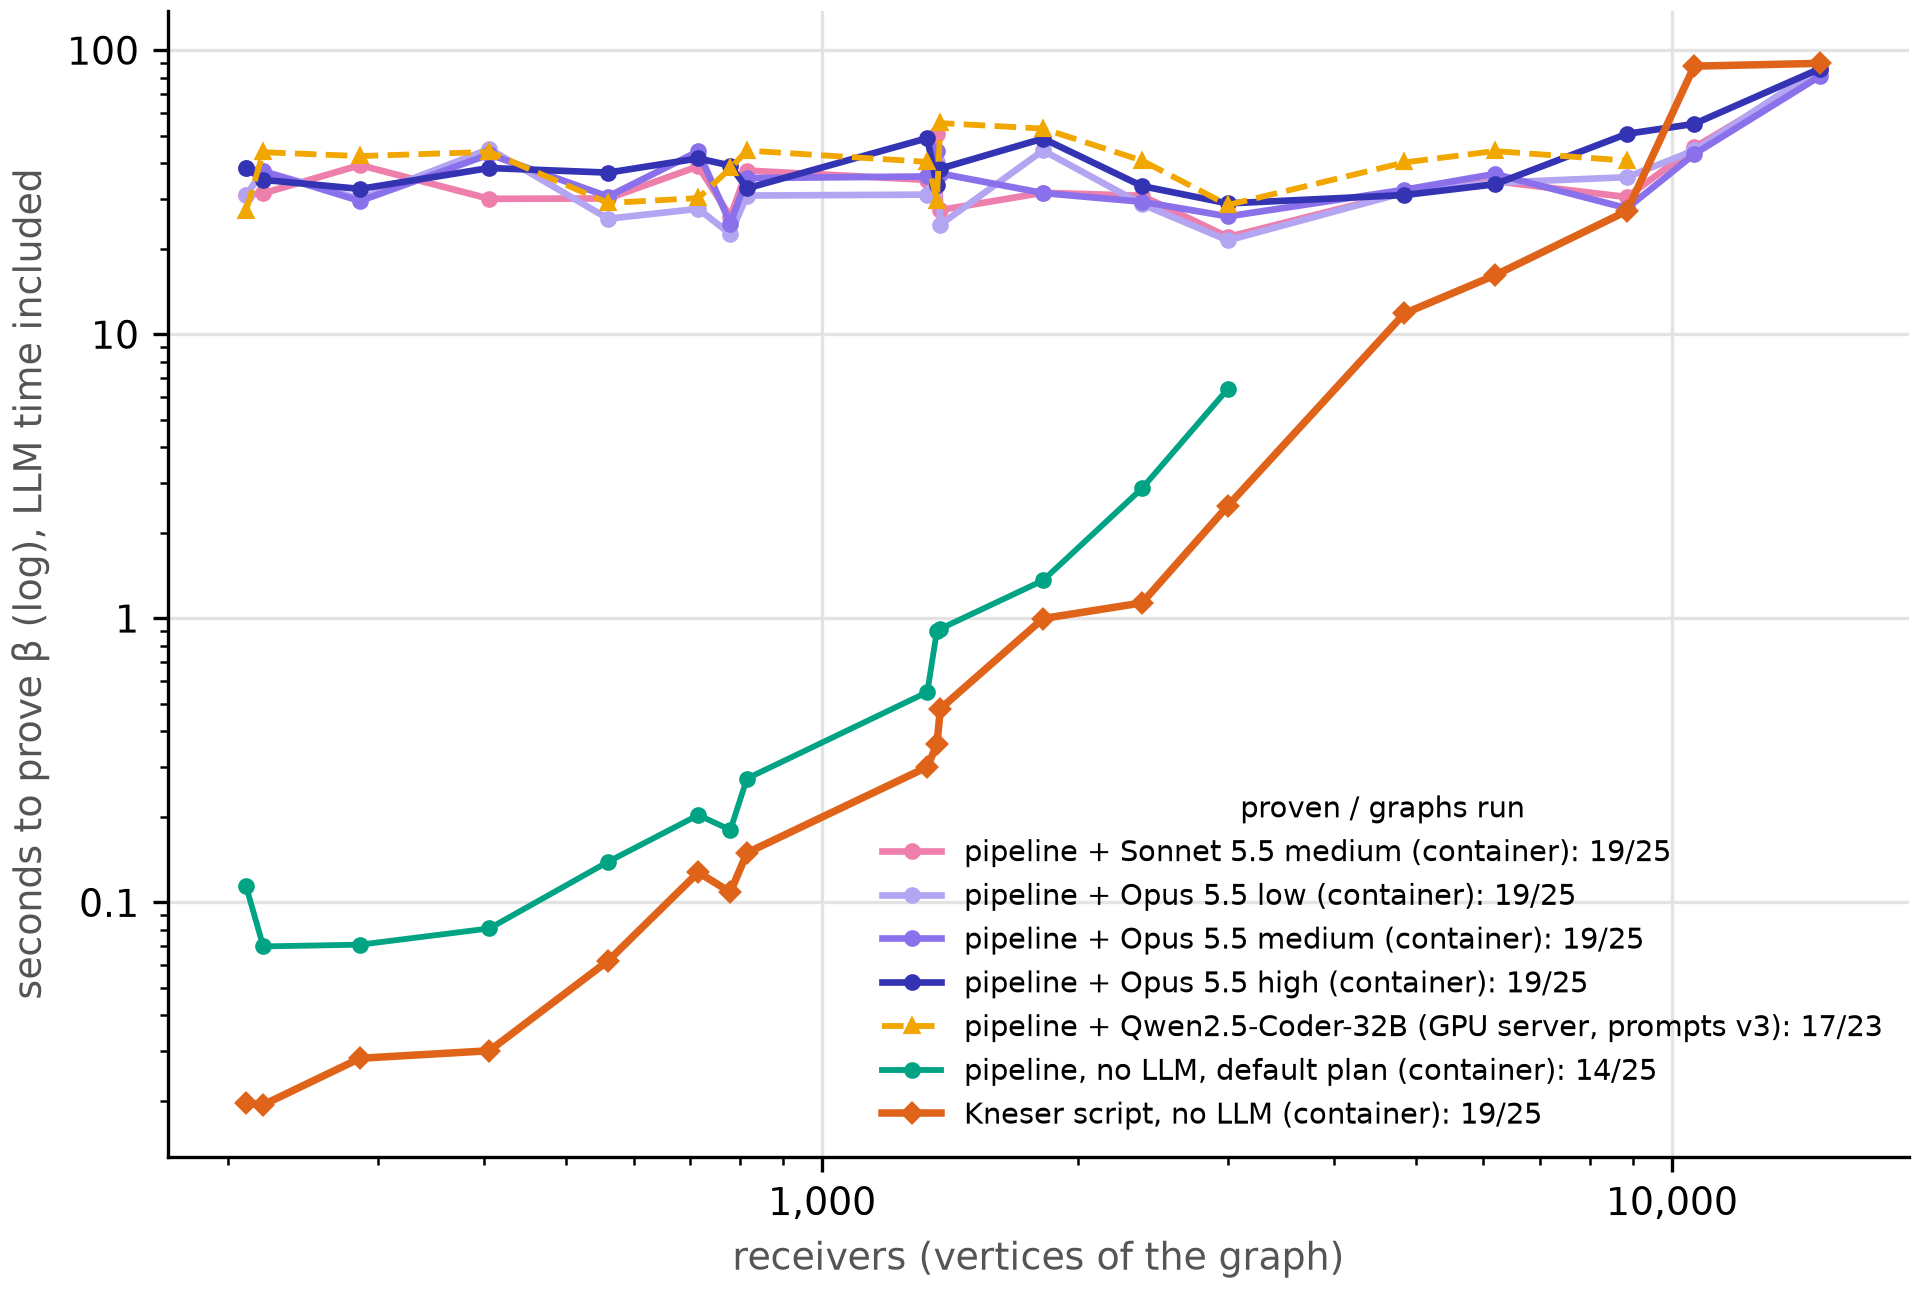
\includegraphics[width=0.78\textwidth]{fig/time_to_prove_models_beamer.png}
  \caption{Time to prove $\beta$ for each LLM driving the pipeline, the pipeline without an LLM, and the Kneser
  script; the legend gives proven graphs out of graphs run. The Claude, no-LLM and script lines use the protocol of
  Figure~\ref{fig:ttp} (container, one core). Qwen ran on the GPU server (vLLM, prompt version v3, cores shared with
  other users) on 23 of the 25 graphs, so its line is not directly comparable.}
  \label{fig:ttp-models}
\end{figure}

\textbf{What the results show, and what they do not.}
\begin{itemize}
  \item All four Claude settings and the Kneser script prove the same 19 graphs; more effort only adds time.
  \item The 6 graphs left open (the 3 exceptions of the theorem and the 3 perturbed or random controls) stay open for
  every method; no method claimed a false value, and every agent bound passed the independent verifier.
  \item \textbf{The LLM's contribution is recognising the family, and code does that too.} Without an LLM, the
  default plan proves the 14 regular Kneser graphs and none of the 5 large ones, because it never calls the family
  rule. With any Claude model the Solver names $K(n,k)$ and the family rule closes all five. But the opt-in fast path,
  a few lines of code with no LLM, recognises $K(n,k)$ the same way and proves every graph it was run on that the
  Claude agents prove (17 of 23). On this benchmark, which consists of Kneser graphs and close relatives, the LLM adds
  no proven graph over that rule and costs a median of 30\,s of LLM time per graph (12--50\,s over the 76
proven Claude runs).
  \item \textbf{The speed on large graphs comes from the rank engine, not the LLM.} The pipeline's rank engine stops
  once the rank is certified ($O(N^2r)$), while the Kneser script computes a full exact rank ($O(N^3)$). With the LLM
  the pipeline needs 43--55\,s at 10{,}626 receivers against the script's 88\,s, of which 28--42\,s is LLM time. The
  no-LLM fast path through the same engine is faster still: it proved $K(20,4)$, $K(17,5)$ and $K(23,4)$ in
  5.2--23.2\,s on 26 November and 2.5--10.0\,s in the 27 November rerun (Section~\ref{sec:gpubench}), against 28--51\,s for the Claude agents in the container; the machines
  differ, so this is indicative, and the fast path was not run at 10{,}626 or 14{,}950 receivers.
  \item \textbf{Where an LLM could matter, we have no evidence yet.} A plan written for the graph at hand should help
  on graphs that no fixed rule recognises. The benchmark has no such graph on which any method closes the bracket, so
  this remains a hypothesis.
\end{itemize}

\textbf{How blind the agent is.} ``Blind'' means only that the input contains no graph name and the vertices are
shuffled. Two limits follow. First, nothing sandboxed the Claude Code agents: the instruction of
Step~R\ref{st:agentrun} told each agent to run one command and read no other file, but no mechanism enforced it, and
an agent could in principle have read the repository (including the benchmark specification). Second, the models
know Kneser graphs from training, and $N=\binom nk$ with degree $\binom{n-k}{k}$ is a strong signature that a model
can match from memory. Recognising the family is therefore not evidence of reasoning about an unknown structure; the
fixed \texttt{binomial\_match} rule does the same. Every bound is still certified by code, so neither limit can make
a reported value wrong; they limit what the agent results say about the LLM.

\subsection{Earlier benchmark on the GPU server (26 Nov, Qwen2.5-Coder-32B)}\label{sec:gpubench}
GPU server, 64 cores shared with other users; baselines pinned to cores 16--27, agent runs to 28--31 (3 workers);
standard methods 120\,s each; agent budget 300\,s. These Qwen numbers use prompt version v3 on code before the plan-step
results were shown to the agents.
\begin{itemize}
  \item Proven exact, 20 benchmark graphs: standard methods 2, the Kneser script 14, agent without LLM 14, agent +
  Qwen 32B 14 (also 14 with generic rules only). All 14 are the regular Kneser graphs.
  \item Large graphs (4{,}845--8{,}855 receivers): the Kneser script 3/3, agent + Qwen with the rule 3/3, agent
  without LLM 0/3, agent + Qwen generic only 0/3, standard methods 0/3. In the default plan the family rule is reached
  only through an LLM hypothesis, and it is what closes these graphs; the opt-in fast path below reaches the same
  rule without an LLM.
  \item Speed: without an LLM the agent is slower than the Kneser script on the shared exact graphs (median time
  ratio \x0.61, by at most 0.6\,s), and \x135 faster than the standard methods on the 2 graphs they prove. On the large
  graphs the agent's compute time is 5--8\x{} lower (2.3 / 4.5 / 8.0\,s against 18.7 / 23.0 / 41.6\,s), but with LLM
  seconds its wall time is about 2\x{} longer on two of them and equal on $K(23,4)$. Qwen adds a median 43\,s of LLM
  time per run (max 56\,s).
  \item Fast path (opt-in, no LLM): recognising $K(n,k)$ from the receiver count and degree and applying the rule
  proves $K(20,4)$, $K(17,5)$, $K(23,4)$: the bracket closed at 5.2 / 15.0 / 23.2\,s on 26 November (the Kneser
  script: 18.7 / 23.0 / 41.6\,s) and at 2.5 / 5.3 / 10.0\,s in a rerun on 27 November (the row of
  Table~\ref{tab:ablation}); times from the run traces. Both are faster than the agent with Qwen and than the Claude
  agents in the container (28--51\,s).
  \item Losses: to the Kneser script, on time, on most small exact graphs (e.g.\ $K(21,2)$ 0.12\,s against 0.03\,s);
  never on accuracy. On the 3 exceptions both reach the same brackets ($[84,93]$, $[286,287]$, $[495,507]$); on the
  controls the agent's brackets are tighter ($K(16,4)$ minus 1\% of edges: $[455,534]$ against $[0,1818]$). The
  script's lower bound of 0 is what it reports, not a bound anyone would accept: on a graph it does not recognise it
  skips its greedy independent set, and its general solver returned no lower bound within the time limit. Any greedy
  independent set gives at least 1, and the agent's gives 455.
\end{itemize}

\subsection{Blind-agent ablation: what the model changes}
\begin{figure}[ht]
  \centering
  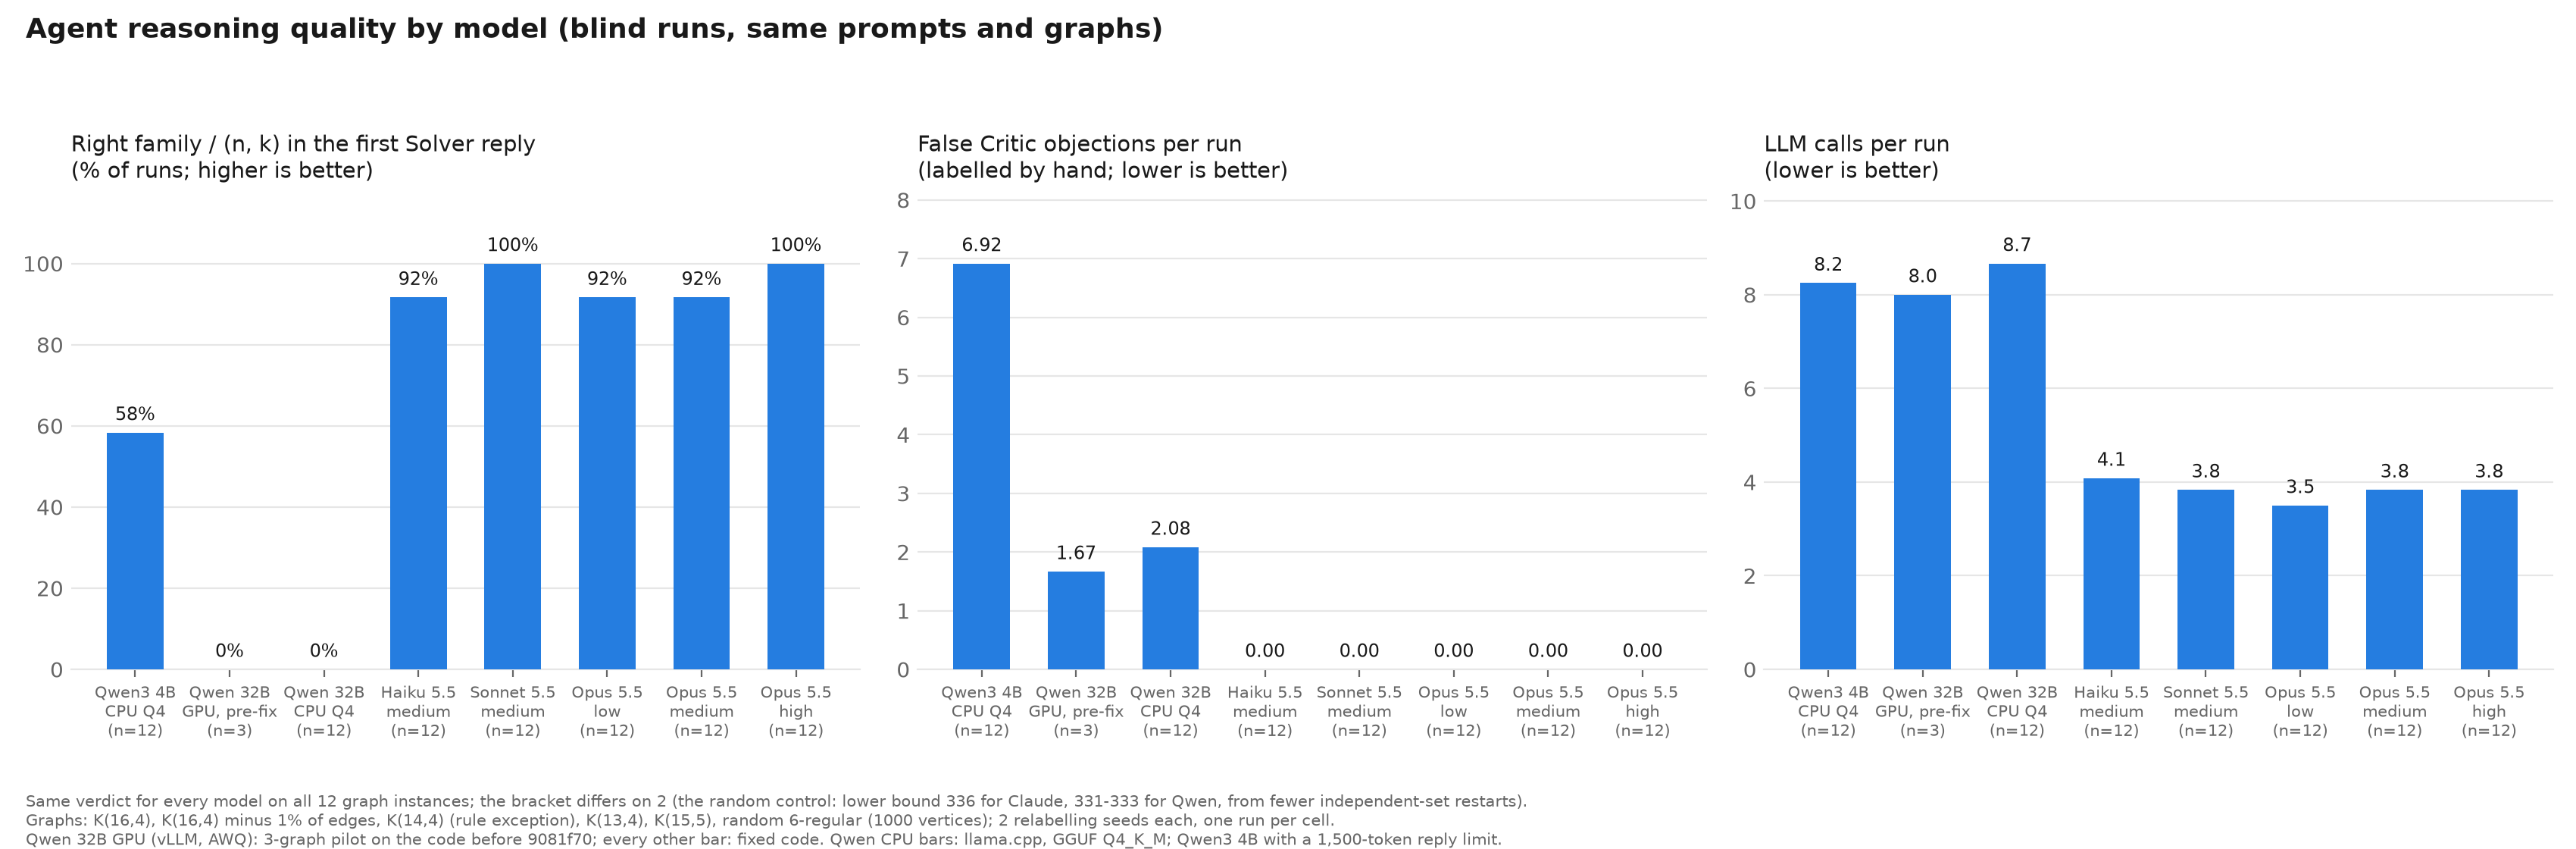
\includegraphics[width=\textwidth]{fig/model_ablation.png}
  \caption{Reasoning quality by model on 6 graphs \x{} 2 relabelling seeds = 12 cells, one blind run per cell:
  $K(16,4)$, $K(16,4)$ minus 1\% of edges, $K(14,4)$ (rule exception), $K(13,4)$, $K(15,5)$ and a random 6-regular
  graph on 1{,}000 vertices.}
  \label{fig:ablation}
\end{figure}

\begin{table}[ht]
  \centering\small
  \begin{tabular}{@{}>{\raggedright\arraybackslash}p{6.4cm}ccc@{}}
    \toprule
    Model & \makecell{False Critic\\objections per run} & \makecell{Right family in\\first Solver reply} & \makecell{LLM calls\\per run} \\
    \midrule
    Claude (Haiku 5.5 medium, Sonnet 5.5 medium, Opus 5.5 low/medium/high) & 0 (in 60 runs) & 11--12 of 12 & 3.5--4.1 \\
    Qwen2.5-Coder-32B (CPU, llama.cpp) & 2.08 & 0 of 12 & 8.7 \\
    Qwen2.5-Coder-32B (GPU pilot, earlier code, 3 runs) & 1.67 & 0 of 3 & 8.0 \\
    Qwen3-4B (CPU, 1{,}500-token limit) & 6.92 & 7 of 12 & 8.2 \\
    \bottomrule
  \end{tabular}
  \caption{Blind-agent ablation (values of Figure~\ref{fig:ablation}).}
  \label{tab:blind}
\end{table}

Every model reaches the same verdict on every graph instance and the same bracket on the 10 Kneser-type instances;
on the random control the lower bound differs (Claude 336, Qwen 331--333) because the Claude Solvers asked for
200--1{,}000 independent-set restarts and Qwen for 10. The model changes the dialogue and its cost, and only through
its plan the bound, never the correctness. Every objection was labelled with a reason by a fixed rule. Qwen3-4B at
the default 600-token limit had its JSON cut off in 26 of 48 requests, hence the 1{,}500-token rerun.
